\documentclass[11pt,letterpaper]{article}
% \usepackage{times}
\usepackage[left=1.75cm,right=1.75cm,top=2cm,bottom=2cm]{geometry}
\usepackage[utf8]{inputenc}
\usepackage[spanish]{babel}
\usepackage{endnotes}
\usepackage{hyperref}
\usepackage{amsmath}
\usepackage{amsfonts}
\usepackage{amssymb}
\usepackage{graphicx}
\usepackage{setspace}
\usepackage[sort&compress]{natbib}

\onehalfspacing

\renewcommand{\notesname}{Notas}

\hypersetup{
    colorlinks=true,
    linkcolor=blue,
    filecolor=magenta,      
    urlcolor=magenta,
    citecolor=magenta,
}

\urlstyle{same}


\let\footnote=\endnote

\providecommand{\keywords}[1]
{
  \small	
  \textbf{\textit{Palabras clave---}} #1
}

\title{%
  Tres Estudios Abiertos \\
  \large Prácticas performáticas, audiovisuales y experimentales en el navegador}

\author{Emilio Ocelotl Reyes}
\begin{document}

\maketitle

\begin{abstract}

\section*{Resumen}

\textit{Tres Estudios Abiertos} es un proyecto de investigación que busca adentrarse en nuevas prácticas experimentales y audiovisuales para el navegador. Parte de la programación de un esqueleto de granulación audiovisual complementado con módulos personalizados de software. Atiende a niveles altos de programación para el control de software por medio de una interfaz de texto. 

Toma en cuenta piezas para el navegador que fungen casos de estudio. El proyecto busca demostrar que las lógicas de los lenguajes de programación posibilitan formas de pensamiento específicos con consecuencias estéticas definidas. 

Los casos de estudio son entramados de audio y pretenden ser ligeros, sin instalaciones, sin referencias a instalación de dependencias de terceros, basados en la web, distribuidos y optimizados para el bajo consumo de recursos de la computadora. 

Hasta el momento considera a \textit{Javascript}\footnote{¿Todavía es posible usar otros lenguajes de programación?} como el lenguaje principal de los casos de estudio. De manera secundaria el proyecto se pregunta si es posible deducir ideas estéticas de las arquitecturas de los lenguajes de programación para la escritura de interfaces textuales de control. 

Adicionamente al estético y tecnológico, consideramos un tercer hilo que corre paralelamente al bucle de investigación-creación: el investigativo. En esta pista están presentes reflexiones e implicaciones políticas en la escritura de y con software.

La investigación busca relacionar la escritura del texto resultante con la escritura de software y otros medios (principalmente repositorios de código pero también imágenes, sitios web, sonido). De esta manera el documento resultante busca desbordarse del papel y de la palabra escrita. 

\end{abstract}


\chapter{Antecedentes}

% este apartado podría tener un orden: de lo más lejano a lo más cercano

% Aquí pienso colocar los antecedentes del proyecto.
% Me pregunto sobre la pertinencia de escribir una especie de estado del arte.
% Había pensado hablar de algunos proyectos cercanos que influyen en el proyecto
% Esto aparece ligeramente enunciado en el artículo de Panorama y en el texto que preparé para el coloquio
% Podría hacer un seguimiento al trabajo que hacen personas cercanas
% Incluso aquí podrían ir los primeros ejercicios en la web 
% Me imagino que aquí podrían aparecer algunos registros anectóticos 

Los antecedentes de esta investigación aluden a una trayectoria que va de la transición de la escritura de software para la realización de sistemas interactivos a la escritura de módulos de software audiovisuales. Estas experiencias toman como premisas la optimización y la ligereza de hardware (por ejemplo, con el uso de computadoras de placa reducida como Raspberry Pi o Jetson Nano ) y la elaboración sistemas ligeros, accesibles y portables para la síntesis y renderización audiovisual en el navegador.

A la par de la práctica artística con tecnología, los elementos precedentes de esta investigación se han conducido hacia la problematización del software como una instancia tanto de conocimiento como de ideas que conforman un paradigma que atraviesa todo el entramado de personas, investigaciones, escritos y obras involucrado con esta actividad. Estas reflexiones han tenido eco en el campo de investigación denominado estudios del software.

Los antecedentes a continuación descritos no necesariamente tienen un orden cronológico o de importancia. En todo caso es un compendio de perspectivas, plataformas, obras y realizaciones prácticas que desde la perspectiva de quien suscribe este texto, son relevantes de enunciar para captar las incidencias en los casos de investigación. 

\section{Música por computadora}

%\subsection{Documenta X} % Pendiente tal vez podría ir en las conclusiones o como una problemmatización een la parte de montaje de anti

%Conexiones y accesos en muestras que implican espacios físicos y digitales. 

\subsection{Plataformas}

A continuación, haremos un breve rastreo de ideas centrales en la escritura de software orientado a la creación musical. El objetivo de este apartado consiste en describir y detectar la presencia del concepto unidad generadora en diversos programas orientados a la generación musical, de entre los cuales está una de las librerías que la presente investigación implementa.

El punto de partida de esta indagación es MUSIC N, proyecto de Max Mathews que sería el parteaguas del paradigma de la música por computadora. Uno de los primeros casos de esta instancia es el principio de programas como Max/MSP y PureData, proyectos representativos de la programación gráfica presente en flujos de trabajo gráfico actuales como TouchDesigner.

Como una observación adicional, es importante detectar instancias de la programación gráfica y de las ideas principales de la música por computadora en plataformas con giros programáticos particulares. Tal es el caso de OpenMusic, que de manera específica está basado en Common Lisp.

Desde la perspectiva de la programación escrita, destacamos el papel que ha tenido SuperCollider en la extensión del paradigma de la música por computadora en la actualidad. Señalamos la importancia de SuperCollider como el motor bajo el cual se pueden ejecutar entornos de programación al vuelo como Tidal Cycles o FoxDot. 

Estuary es un caso adicional que permite establecer un puente entre Tidal Cycles como un entorno que ejecuta SuperCollider como motor de audio y el navegador como tecnología multiplataforma sin instalaciones. Esta plataforma utiliza secuenciadores basados en la sintaxis de Tidal Cycles pero a diferencia del entorno que se puede instalar de manera local en una computadora, Estuary utiliza al navegador como motor de audio. 

Trazamos estas relaciones para establecer una relación continua y presente entre los entornos anteriormente descritos y una de las librerías utilizadas en los casos de estudio de esta investigación: Tone.js. En este sentido, consideramos importante la adscripción a los principios de la música por computadora para encontrar soluciones personalizadas para el navegador.

\subsection{Jacktrip y la música conectada}

raspis conectadas y jacktrip > el trabajo realizado por CCRMA y en general 

La labor del colectivo Radiador

La radio y la transmisión de sonido con Icecast 

Sonobus y la resolución de problemas de streaming en tiempos de pandemia

El caso del ensamble y la propuesta de talleres de la gira del colectivo RGGTRN 

\subsection{Fluxus y openGL}

Para el caso de la imagen, retomo la influencia que tiene en la comunidad de live coding y en mi experienciación del performance audiovisual con la computadora el papel que tuvo el desarrollo Fluxus\footnote{\url{https://gitlab.com/nebogeo/fluxus/}} de Dave Griffiths que se remonta al 2007. Detrás de Fluxus también cabe destacar la importancia de sistemas de renderización de gráficos por computadora como OpenGL, que actualmente, son el punto de partida de software de alto nivel involucrado con este proyecto como OpenFrameworks y la variante para el navegador, webGL, que implementa la librería Three.js 

% Pregunta, esto no tendría que ir en otros momentos? Tal vez disperso o tal vez en la introducción 


\section{Trilogía de Investigación}

\textit{Tres Estudios Abiertos} forma parte de una trilogía de investigación.

\subsection{Objeto, Paisaje y Efecto}

La primera parte fue Objeto, Paisaje y Efecto \citep{ocelotlLic}, un proyecto de investigación que abordó las nociones de objeto sonoro \citep{schaeffer}, paisaje sonoro\citep{schafer1} y efecto sonoro \citep{augoyard} para considerar a la escucha como un recurso para la investigación sociológica en música y para la investigación social desde el sonido.

\subsection{Cuidado con la Brecha}

Un segundo punto de investigación involucró un proceso de investigación-producción artística \citep{ocelotlMas}. La realización de este proyecto fue un prototipo tecnológico y partió de objetivos que inicialmente estaban propuestos como secundarios pero que más tarde se revelaron como parte del núcleo en la investigación. Estos aspectos son: 1) el proceso de trabajo colaborativo y su implementación con herramientas como git, 2) la reflexión sobre la interacción entre audio e imagen en la composición musical electroacústica y 3) el uso de herramientas libres, personalizadas para la realización de prototipos audiovisuales y para el planteamiento de una observación crítica de procesos creativos donde investigador y artista son el mismo agente. La propuesta de los estudios del software fue incorporada en este momento de investigación. 

\subsection{Tres Estudios Abiertos}

Referencia recursiva a esta investigación para explicar la trilogía


\section{Live Coding}

% Antecedentes más extensos

\subsection{Primeras expresiones}

Antecedentes del live coding: la escena mod.

En el manifiesto del live coding se expresan pensamientos que hasta el momento, son vigentes. 

% PhD Thesis: Artist-Programmers and Programming Languages for the Arts - Alex McLean 
Dentro de los antecedentes está la experiencia performática de escribir código al vuelo con fines creativos, audiovisuales y experimentales.

Las primeras expresiones reflexivas y prácticas del live coding no solamente establecen puntos de partida performáticas, sino que al mismo tiempo aportan elementos para el diseño y análisis de sistemas basados en interfaces de código:

\begin{quote}

  ``Nuestro argumento nos lleva a través de capas de representación, comenzando con símbolos, luego palabras, lenguaje y notación, para considerar el papel que estas representaciones pueden jugar en la creatividad humana'' \citep[p.~3]{McLean2011}

\end{quote}

  
La noción de capas de representación permite analizar la complejidad del proceso artístico con código en términos de la relación entre humanos y los aspectos cognitivos, sociales y políticos que les atraviesan, y los no-humanos en lo que respecta a las posibilidades de conocimiento instanciado presentes en ellos. 

Live coding desde cero y la improvisación. 

\subsection{Nodos y circuitos}

La práctica de la programación al vuelo, delimitada técnica, escénica, musical y visualmente se origina en Inglaterra. % cita

Como lo describen \cite{villasenor} para los casos de Barcelona y Ciudad de México.\footnote{Un ejemplo reciente se encuentra en: \url{https://youtu.be/n5kwi4eRAE4}} 

\subsection{Exploración visual}

Exploración visual para la integración con el sonido.  

\begin{figure}[tb]
\centering 
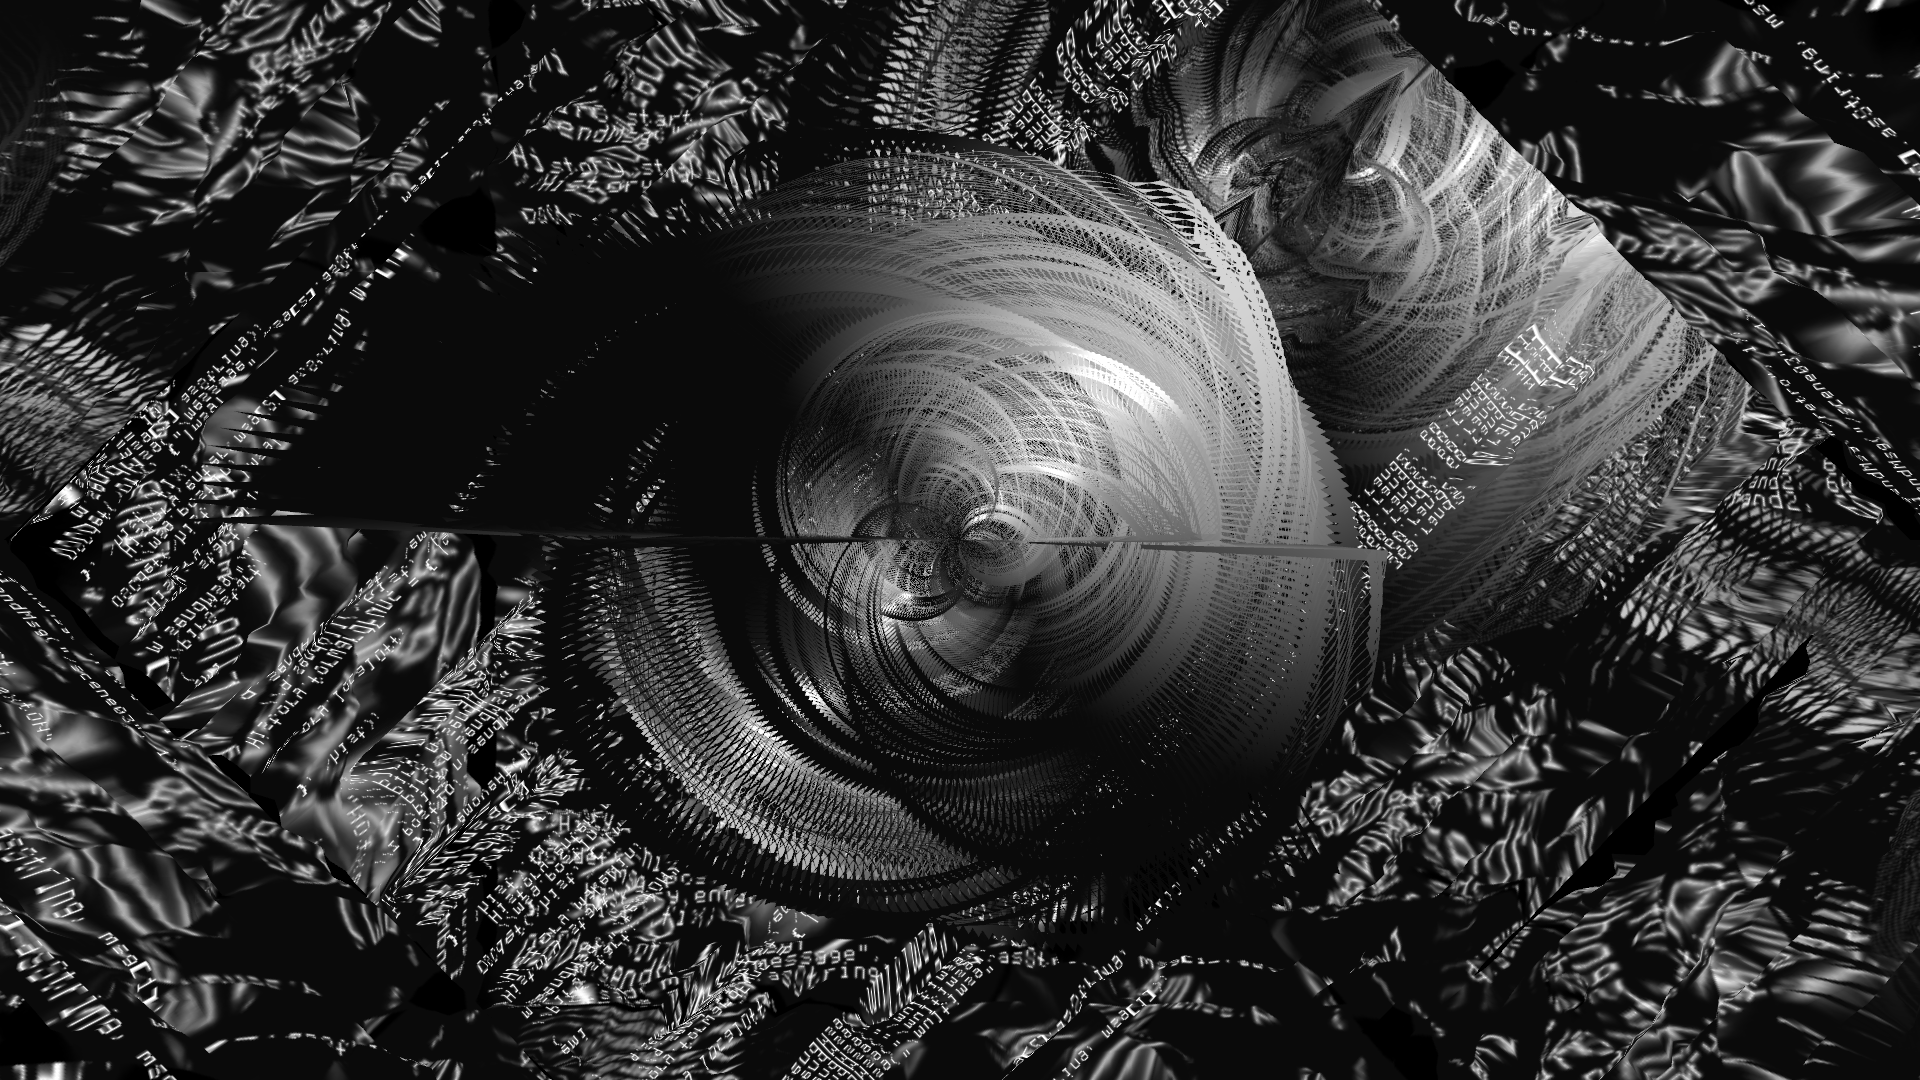
\includegraphics[width=\columnwidth]{img/of13.png} 
\caption[Openframeworks 1]{Captura de render realizado con OpenFrameworks} % The text in the square bracket is the caption for the list of figures while the text in the curly brackets is the figure caption
\label{fig:gallery} 
\end{figure}

El campo del live coding tuvo un giro importante con la llegada de hydra de Olivia Jack. La rápida expansión de esta plataforma y la sintaxis que recuerda la conexión de flujos de energía similar a los sintetizadores analógicos favorecieron la producción de piezas e interpretaciones enfocadas en la imagen y en algunos otros casos a la par del audio. La importancia de esta plataforma ha delimitado una estética  basada en  la transformación de píxeles, de formas y de transformaciones basadas en funciones matemáticas.

En palabras de Olivia Jack, los procesos que realiza la computadora hay un eje de profundidad, en términos del despliegue gráfico físico de la computadora de espacios bi o tridimensionales, el resultado es bidimensional.

La lógica de Hydra es modular, esto quiere decir que puede incorporarse como un componente adicional a proyectos que no necesariamente se centren en la producción visual con esta plataforma. Esta modularidad juega a favor de lenguajes de programación como Javascript. 

\section{Proyectos Colindantes}

Algunos proyectos cercanos tecnológica, conceptual y estéticamente a \emph{Tres Estudios Abiertos} son: 

\subsection{Nivel Bajo}

\begin{itemize}

\item Ruffbox\footnote{\url{https://github.com/the-drunk-coder/ruffbox}}
\item WebAssembly/Rust Tutorial\footnote{\url{https://www.toptal.com/webassembly/webassembly-rust-tutorial-web-audio}}
\item Flocking\footnote{\url{https://github.com/continuing-creativity/Flocking/}}
\end{itemize}

\subsection{Nivel Medio}

\begin{itemize}

\item supercollider.web\footnote{\url{https://github.com/khilnani/supercollider.web/}}
\item Web Audio API\footnote{\url{https://developer.mozilla.org/es/docs/Web/API/Web_Audio_API}}
\item Tone.js\footnote{\url{https://tonejs.github.io/}}
\item SuperCollider.js\footnote{\url{https://github.com/crucialfelix/supercolliderjs/}}
  
\end{itemize}

\subsection{Nivel Alto y Ecosistemas}

\subsubsection{Nivel Alto}

\begin{itemize}
\item Hydra\footnote{\url{https://github.com/ojack/hydra}}
\item Troop\footnote{\url{https://github.com/Qirky/Troop}}
\item flok\footnote{\url{https://github.com/munshkr/flok}}
\item tilt\footnote{\url{https://github.com/munshkr/tilt}}
\item LiveLab\footnote{\url{https://github.com/ojack/LiveLab}}
\item timeNot\footnote{\url{https://github.com/luisnavarrodelangel/seis8s}}
\item seis8s\footnote{\url{https://github.com/AFrancoB/timeNot}}
\item Camposonico\footnote{\url{https://github.com/diegovdc/camposonico}}
\item INSTRUMENT\footnote{\url{https://github.com/punksnotdev/INSTRUMENT}}
\end{itemize}


\subsubsection{Ecosistemas}

\begin{itemize}
\item Estuary\footnote{\url{https://github.com/dktr0/estuary}}
\item Sema-engine\footnote{\url{https://github.com/frantic0/sema-enginef}}
\end{itemize}

\section{Piezas y obras lejanas}

\subsection{Notas de Ausencia} % Cambiar la redacción para que no sea exactamente igual al artículo de panorama 

Notas de Ausencia de Marianne Teixido  es un ensayo generativo en la web. Utiliza texto-dato que por medio de la computadora como agente resignificante, deconstruye estructuras discursivas para resemantizar la narrativa sobre las desapariciones de mujeres en México y América Latina.

El tiempo y espacio virtual conforman una partitura para la memoria y la denuncia. La narrativa, semi-autónoma, argumenta a partir de textos tomados de tweets, poemarios, libros y artículos feministas que explican desde la teoría las desapariciones forzadas, el feminicidio y la violencia de género. Estos elementos están presentes como texto, imagen y sonido en un espacio tridimensional diseñado a manera de memorial.

La narrativa de la pieza está articulada mediante la intervención de dos bots que interactúan en Twitter. El primero realiza una búsqueda de tuits a partir de un filtro de palabras clave escritas como hashtags como: \#MéxicoFeminicida, \#MadresEnBúsqueda, \#ViolenciadeGenero, \#NiUnaMenos, entre otros.\footnote{Al momento de escritura, el bot se encuentra activo en la cuenta: \url{https://twitter.com/notasausencia} (Consultado el \today} Posteriormente, recomparte el tuit que contiene alguno de los hashtags de la base de datos previamente delimitada. El segundo bot retoma los textos de los tuits seleccionados y los remixea para generar un segundo texto automático por medio de cadenas de Markov.

Esta pieza se realizó en el contexto de la exhibición en línea Creaciones con Algoritmos: Visualización y Sonificación de Datos del Centro de Cultura Digital en abril de 2020. Su salida oficial se realizó en video sin embargo, el planeamiento original contempló la creación de un espacio virtual en la web que pudiera visualizar en tiempo real la información viva proveniente de los tweets.

Dos características definieron el diseño de la pieza: ubicación de la pieza en un espacio tridimensional y la interacción y visualización de la información proporcionada por los bots. Para la realización, el proyecto retomó módulos iniciales de Panorama y partió del uso de Three.js como un entorno de trabajo que pudiera conectar los dos momentos de la pieza antes descritos.

\subsection{Visuales, Hydra y P5.js}

Uno de los referentes en términos de live coding con resultados visuales es la obra de Olivia Jack. La realización de éstas va de la mano con el software desarrollado por ella misma: Hydra. El proyecto está alojado en la web y la descripción se define como: ``[U]na plataforma para live codear visuales, en la que cada ventana del browser puede ser usado como un nodo de un sintetizador de video, modular y distribuido'' \footnote{Consultado el \today en: \url{hydra.ojack.xyz}}

Hydra es un proyecto abierto y libre, lo cual permite que una comunidad de usuarios se involucren en el uso, mantenimiento y expansión del repositorio. Algunos proyectos que utilizan directa o indirectamente hydra. 

\subsection{The Stage is (A)Live}

The stage is (a)Live\footnote{\url{https://www.geometries.xyz/theStageIsAlive/}} - Johana Chicau y Renick Bell

\section{Piezas y obras cercanas} % Pendiente, igual y no hay tantas cosas 

\subsection{Pumpumyatchkan}

\subsection{Concierto de clausura}

Concierto virtual realizado en el marco del coloquio de alumnas del Programa de Postrado en Música de la UNAM

\begin{figure}[tb]
\centering 
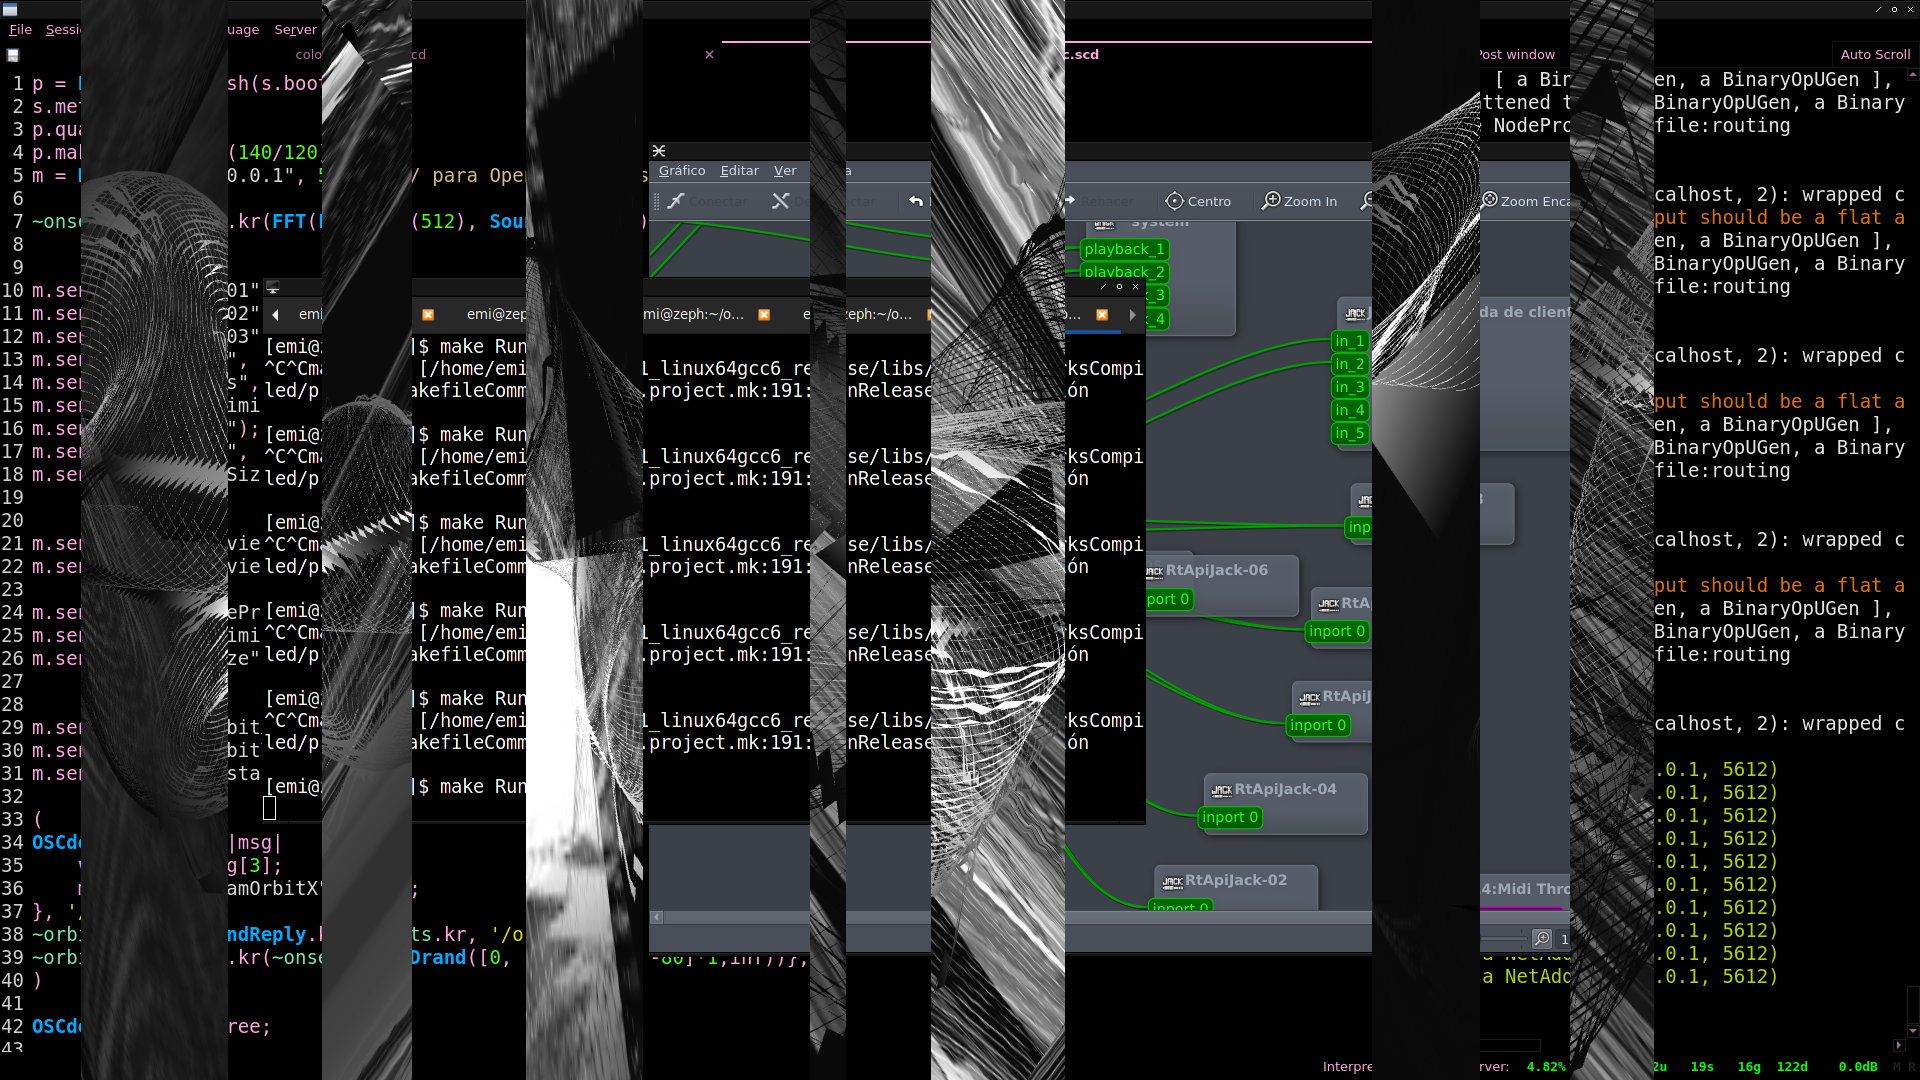
\includegraphics[width=\columnwidth]{img/col2.png} 
\caption[Concierto coloquio]{Captura del concierto del Coloquio de alumnas \url{https://youtu.be/HwBTRQKr9Ps}.} % The text in the square bracket is the caption for the list of figures while the text in the curly brackets is the figure caption
\label{fig:gallery} 
\end{figure}

\section{PiranhaLab}

Otro antecedente de este proyecto es la práctica y reflexión planteada en colectivo por\textit{PiranhaLab}\footnote{``PiranhaLab es un laboratorio interdisciplinario que trabaja en las tripas del software''. \url{https://piranhalab.github.io/} (Consultado el \today)}.

\subsection{Escritura de y con software}

\subsection{Ciclo de Talleres}

El ciclo de talleres realizado en el Centro de Cultura Digital (CCD) en coparticipación con el Laboratorio de Tecnologías Libres\footnote{Actualmente Laboratorio de Tecnologías Compartidas} permitió plantear dos conclusiones que se heredan a \textit{Tres Estudios Abiertos}: La difuminación de la distinción usuario/desarrollador como una motivación para la escritura de software y la procuración de diversidad en la escritura de software en América Latina.

\begin{figure}[tb]
\centering 
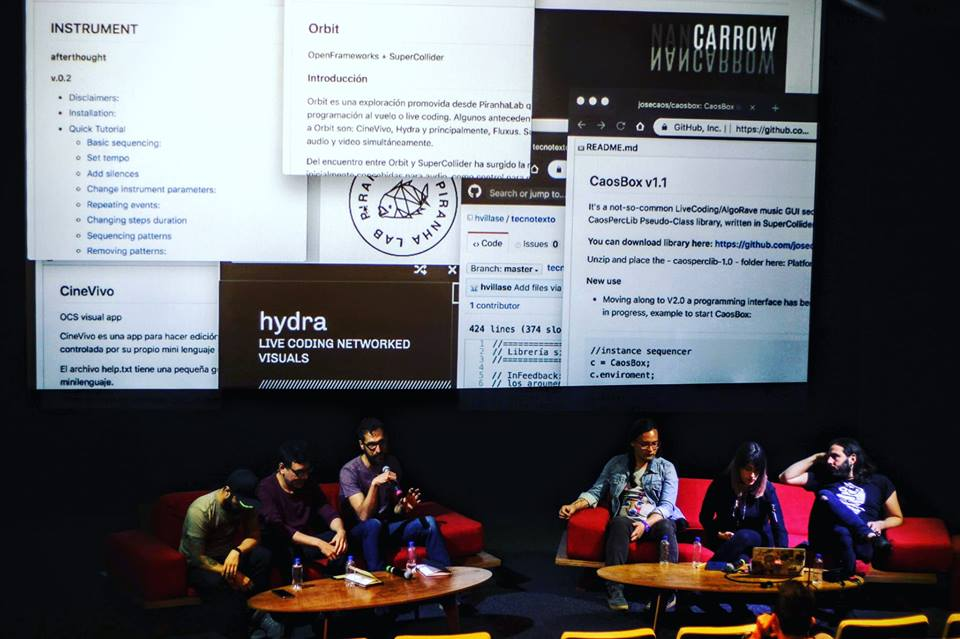
\includegraphics[width=\columnwidth]{img/conversatorio.jpg} 
\caption[Conversatorio CCD]{Conversatorio organizado por PiranhaLab y el Laboratorio de Tecnologías Compartidas en el CCD. 2019.} % The text in the square bracket is the caption for the list of figures while the text in the curly brackets is the figure caption
\label{fig:gallery} 
\end{figure}

\subsection{EDGES 2020}

La escritura de espacios para el ciclo de conciertos EDGES 2020 realizado por el Taller de Imágenes en Movimiento del Centro Multimedia (CMM) permitió la exploración de entornos tridimensionales inmersivos en el navegador en el contexto del encierro causado por la pandemia de COVID-19. Técnica y conceptualmente la escritura de estos espacios digitales influye en el presente proyecto. El artículo \textit{Panorama} \citep{panoramaArticulo} hace referencia de manera extensa al ecosistema de espacios y propuestas que también inciden en \textit{Tres Estudios Abiertos}.

% Esto se articula con las actividades colectivas de la sección casos 

Espacios inmersivos que estuvieron activos de manera simultánea. 

\printendnotes
 %% Esta es la parte más fuerte de la investigación
\section*{Premisa y objetivos}

% Partimos del bucle de investigación-creación para reducir la brecha de la escritura y la investigación sobre y con software. > Esto va en metodología según yo 

La premisa principal de la investigación consiste en estudiar casos específicos de programación estética orientada a la integración audiovisual, posibilitada a partir de lenguajes de programación y observada desde bucle investigación-creación. 

De esta premisa se desprenden los objetivos secundarios: escribir software que pueda ser implementado en el contexto de obras audiovisuales para el navegador y realizar reflexiones a manera de documentación que vinculen conceptos tecno-sociales y estéticos. 


\section*{Plantamiento del problema}

De entre los proyectos similares destacamos aquellos que son de Nivel Alto para responder a la pregunta: ¿Cuál es la diferencia entre los proyectos mencionados y \textit{Tres Estudios Abiertos}? Dos perspectivas podrían aclarar el punto de partida del proyecto. La primera es funcional y hace referencia a la solución de problemas partiendo de una comunidad que ejecuta, retroalimenta y enriquece al proyecto. La segunda, apuesta por la diversidad en el desarrollo de interfaces de control y que se manifiesta de una manera muy específica en el proyecto Estuary. El presente proyecto busca responder en un momento anterior a la realización de módulos de software si hay diferencias estéticas heredadas de notaciones musicales y computacionales, lenguajes de programación,  estilos musicales, flujos de voltaje que desembocan en síntesis de audio / imagen e incluso planteamientos críticos sobre decolonialidad. Referimos a este conjunto de diferencias como decisiones de diseño en sintaxis de control que tienen consecuencias en la estética que resulta de controlar motores de audio y video. En este sentido, \textit{Tres Estudios Abiertos} es una búsqueda que orbita en estas desiciones y se adscribe a la diversidad en la escritura de y con software. 


% algo tipo metodología

\section*{Escritura y Ejecución}

Para su ejecución, el proyecto alude a la investigación artística y extiende la idea de \textit{loop} o bucle para hablar de la relación que existe entre investigación y práctica artística cuando el investigador y artista son la misma persona, tal y como describe \cite{ocelotlMas}. Esta forma de trabajo retroalimenta la escritura investigativa con la práctica artística y viceversa. Consideramos que esta perspectiva revela aspectos que el distanciamiento convencional no toma en cuenta.

Abordamos procesos artísticos que involucran música, software y computadoras. La investigación no busca realizar mediciones para establecer parámetros de ligereza o eficacia el software resultante. En todo caso, aprovecha la lógica tecnológica de la programación y del procesamiento de información para encontrar soluciones para la investigación y la reflexión.

Rescatamos el uso del repositorio como una estrategia para escribir software, como un respaldo para el trabajo colaborativo y como una documentación que puede modificarse y consultarse en el tiempo. Para la presente investigación, la noción de repositorio de código es central ya que nos permite adentarnos en \textit{las tripas del software} y contemplar al código como un recurso de y para la investigación. En este sentido la escritura y la consulta de software puede realizarse con sistemas distribuidos de control de versiones como \textit{Git}\footnote{``\textit{Git} es un sistema distribuido de control de versiones libre y abierto diseñado para tratar con todo, desde proyectos pequeños hasta proyectos muy grandes con velocidad y eficiencia.'' \url{https://git-scm.com/} (Consultado el \today)}. Con esto, nos adentramos en la discusión sobre el carácter efímero del software y de piezas artísticas para el navegador. 

Aprovechamos la lógica de estos sistemas para construir un entramado que pueda dar cuenta, por un lado, del proceso creativo con los respositorios de las piezas que existen en la web y por el otro, el texto que conforma la investigación y que pretende discutir con la contraparte programada. De esta manera, los procesos quedan lo suficientemente abiertos como para interrelacionarse sin perder delimitación y diferenciación. Buscamos extender la propuesta de un momento anterior de investigación que anuncia la lógica del trabajo con sistemas distribuidos para la investigación artística con tecnología orientada a la creación audivisual.

La ejecución de la investigación consiste en relacionar código, texto y recursos multimedia. En un momento futuro, ponderaremos la implementación de distintos sistemas de escritura de texto/código y elegiremos el que mejor se adapte a los objetivos y alcances del proyecto. Hasta el momento, la investigación considera tres sistemas que de alguna u otra manera se relacionan con la escritura de texto/código: \textit{LaTeX}\footnote{LaTeX es un sistema de composición tipográfica de alta calidad; incluye funcionalidades diseñadas para la producción de documentación técnica y científica. \url{https://www.latex-project.org/} (Consultado el \today)}, \textit{Git} y \textit{JupyterLab}\footnote{\textit{JupyterLab} es un entorno de desarrollo interactivo basado en la web para \textit{notebooks} de \textit{Jupyter}, código y datos. \url{https://jupyter.org/}. (Consultado el \today)}. La elección o combinación de entornos para la escritura de la tesis requerirán una ponderación que tome en cuenta la integración entre texto, código y acoplamiento con el lenguaje de programación principal del proyecto: \textit{Javascript}. De manera complementaria, la investigación contemplará los alcances de diseño, composición tipográfica y estilo personalizados. Como una alternativa al formato de presentación impreso (digital o físico), el proyecto busca que el proceso y el resultado pueda ser compilado y consultado en línea como una página web.\footnote{Una prueba de esta propuesta se puede consultar en: \url{https://emilioocelotl.github.io/tres-estudios-abiertos/}}

La ejecución de la investigación coincide con los planteamientos y la delimitación del proceso de reflexión-creación: estos procesos implican múltiples hilos que corren al mismo tiempo y que podemos enunciar de manera general como: tecnológico, estético y de investigación. El uso de conceptos que atraviesen estos rubros nos permitirá desplazarnos a partir de la retroalimentación que se genera entre tecnología y propuesta artística. El vínculo hacia lo reflexivo puede establecerse en las plataformas para escribir código como entornos de desarrollo integrados (IDEs) y sistemas de control de versiones, en la escritura por sí misma como tecnología y en el uso de conceptos y su vinculación con la metáfora. 



\subsection*{Avances}
 % Funcionaría como resultados
\chapter{Conclusiones}

% Qué papel tienen las "ciencias del espíritu" de cara a la investigación artística que se centra en un tivo de investigación de las "ciencias exactas / naturales" ? 


%% ¿Qué? En el otro docu esto es el planteamiento del problema 
%% ¿Cómo? Metodología 
%% ¿Por qué? Para qué? Igual y esto podría ir en las conclusiones 
%% Conclusiones 

% \nocite{ocelotlMas}

\singlespacing

% \newpage

\theendnotes

\addcontentsline{toc}{chapter}{\protect\numberline{}Referencias}%
\bibliography{../../bib/panBib}{} 
\bibliographystyle{../../bib/apalike-es}

\end{document}
